\section{Componentes generales de las tablas de dispersión}
\label{sec:comp-gener-de}

Hemos visto, como estructura de contenedor, los arreglos y los
árboles, cada uno con sus propias ventajas y desventajas.  Por un lado
los arreglos lexicográficos con una gran eficiencia de acceso, y
por otro, los árboles con el dinamismo y optimización en el uso de la
memoria.  ¿Y si pudieramos tener una estructura que combine las
ventajas de los arreglos lexicográficos y árboles?

Esa es la idea principal de los proponentes de las tablas de
dispersión, por un lado se tiene una tabla representada en una arreglo
lexicográfico, que puede tener elementos dinámicos para crecimiento a
futuro.

Los componentes general de una tabla de dispersión se resumen en la
siguiente gráfica.

\begin{center}
  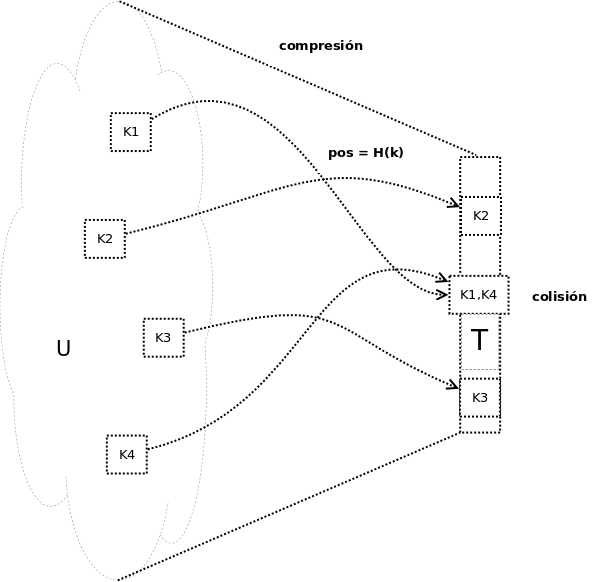
\includegraphics[scale=.35]{1.png}
\end{center}

Podemos distinguir los siguientes elementos:

\begin{itemize}
\item Hay un universo U de elementos posibles que pueden llegar a ser
  utilizados en la memoria
\item Tenemos la tabla T, que es un arreglo lexicográfico en la
  memoria de la computadora, con los elementos de U, realmente
  utilizados
\item Los elementos de U están identificados por llaves $k_i$
\item Las llaves de cada elemento son mapeadas a posiciones
  individuales por medio de una función de dispersión ( \textbf{pos =
    h(k)} )
\item Dado que las llaves $k_i$ pueden ser alfanuméricas, puede existir
  primero una conversión de alfanumérico a numérico.  Este proceso de
  conversión y mapeo puede ser considerado dentro de la misma función
  de dispersión \textbf{h(k)}
\item Dado que \textbf{U $>>$ T} (hay muchos más elementos en \textbf{U}
  que en \textbf{T}) invariablemente se dará el caso en que dos llaves
  mapearán a la misma posición.  Ésto es una \textbf{colisión}.
\end{itemize}

\section{Políticas de resolución de colisiones}
\label{sec:polit-de-resol}

Además de la función de dispersión H(K), el otro componente de las
tablas de dispersión es la política de resolución de colisiones.

Esta política se refiere a la estrategia que se usará para resolver el
problema de las colisiones, que inevitablemente se dará, dado el hecho
que el número de elementos posible en el universo, es mucho mayor que
el número de elementos que caben en la tabla en memoria.

La elección de la política de resolución es tan importante que
normalmente esta decisión da nombre a la estructura, como veremos en
las siguientes secciones.  

\section{Dispersión por encadenamiento}
\label{sec:disp-por-encad}

La forma más simple, es que cada posición de la tabla tiene un
apuntador a una lista que contiene todos los elementos que
colisionaron en esa posición, así:

Esta estrategia tiene la ventaja que es relativamente simple de
implementar, sin embargo su rendimiento, O(n), varía entre
\textbf{n/m} y \textbf{n}. Donde \textbf{n} es el número de elementos
en la tabla y \textbf{m}.

El rendimiento está dado así porque, en el mejor de los casos, en que
la función de dispersión cumple con repartir uniformente los elementos
en la tabla, las listas en cada posición, en el largo plazo, tendrán
la misma cantidad de elementos (\textbf{n/m}).  El acceso a una
posición de la tabla está dado por la ejecución de H(k), lo que se
toma como O(n)=1, y la búsqueda en una lista esta dado por el tamaño
de la lista, por lo tanto O(Tabla.get(k)) = n/m.

Sólo en el caso extremo, en que todos los elementos colisionen en la
misma posición, el rendimiento se degenerará a O(n)=n, dado que todos
los elementos de la tabla estarán en la misma lista.

En busca de optimizar dicho rendimiento, se ha pensado en utilizar
árboles AVL en vez de listas.  Esto implica que O(n) = lg (n/m).  Otra
vez, debido a que los árboles tenderán a tener la misma cantidad de
elementos: n/m.

De forma similar, si usaramos árboles B[k], tendríamos un rendimiento
O(n) = logk(n/m).

En general, cualquier estructura dinámica que se use para resolver la
colisión, el efecto es que el rendimiento se multiplicará, dado que es
más eficiente buscar en una lista o árbol de tamaño \textbf{n/m} que
en una lista o árbol de \textbf{n}, si no usaramos una tabla de
dispersión.

\section{Direccionamiento abierto}
\label{sec:direcc-abierto}

Al contrario del encadenamiento, no utiliza memoria adicional a la
tabla en sí.  Las colisiones se resuelven dentro de la misma tabla,
así:

\begin{center}
  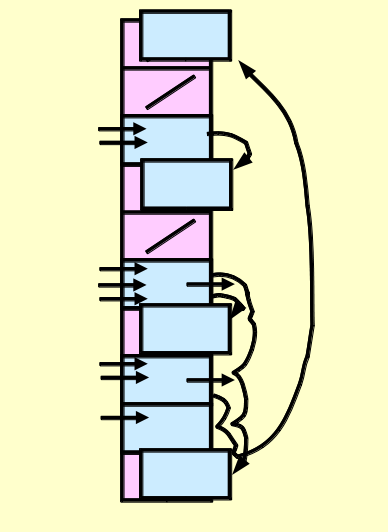
\includegraphics[scale=.5]{3.png}
\end{center}

Básicamente, cuando una llave colisiona en una posición, se sigue la
siguiente estrategia:
\begin{itemize}
\item Se realiza un ciclo de intentos de buscar una posición al elemento
  \begin{itemize}
  \item En cada intento se examina la posición dada por
    \textit{posición actual + S(k,i) \% m} , donde \textit{k} es la
    llave a insertar, \textit{i} es el número de intento y
    \textit{S(k,i)} es la función que determina la \textbf{secuencia
      de prueba}.
  \item Si la posición examinada esta libre, entonces se asigna dicha
    posición y se finaliza
  \end{itemize}
\end{itemize}
    
Según la naturaleza de \textit{S(k,i)}, puede ser que los intentos
generen un ciclo infinito de intentos, por lo que debe establecer un
límite al número de intentos. Dicho límite establecerá el rendimiento
máximo de la estructura.  Diferentes autores han propuesto diferentes
límites, que van desde \textit{m/e} hasta \textit{2m}, donde e es la
constante de Euler.  Esto dependerá del diseñador de la estructura.

\textit{S(k,i)} determinará el comportamiento de la política, que
puede ser:
        
\begin{description}
\item[Lineal: ] \textit{S(k,i)=1}, lo que significa que se examinarán
  posiciones continuas a la posición de colisión.  Ésto provocará que
  se formen grupos de llaves continuas que irán creciendo conforme se
  inserten más llaves.  Ésto se denomina agrupamiento primario.
\item[Cuadrática: ] $S(k,i)=i^2$ creará secuencias de pruebas con saltos
  de la forma 1, 4, 9, 16,.... a partir de la posición de colisión.
  Ésto elimina el agrupamiento primario, pero provoca que todas las
  llaves que colisionan en una misma posición, sigan la misma
  secuencia de prueba, lo que se denomina agrupamiento secundario.
\item[Doble dispersión: ] \textit{S(k,i)= ( k \% c +1 ) * i}.  Se
  utiliza una segunda función de dispersión (por ejemplo \textit{k \%
    c +1} ) lo cual agrega una variación de una llave a otra, por lo
  que, aunque dos llaves colisionen en la misma posición, seguirán
  secuencias de prueba distintas.
\end{description}

\begin{center}
  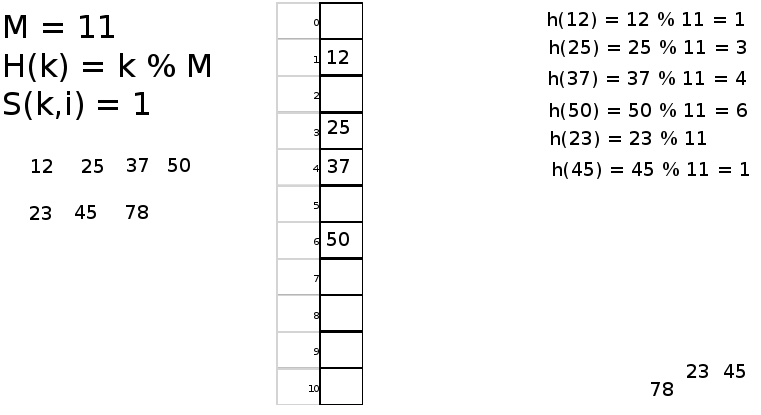
\includegraphics[scale=.4]{4.png}
\end{center}

\begin{center}
  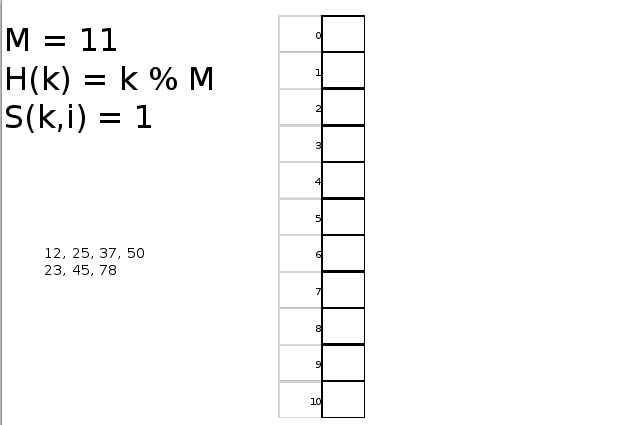
\includegraphics[scale=.4]{5.png}
\end{center}

%%% Local Variables:
%%% TeX-master: "cdc"
%%% End:
